\documentclass[svgnames]{beamer}

\usetheme{Madrid}
\usecolortheme{seahorse}
\usepackage{multirow}
\usepackage{amsthm}
\newcommand{\mn}{\mathbb{N}} %math N%
\newcommand{\mz}{\mathbb{Z}} %math Z%
\newcommand{\bG}{\boldsymbol{G}}
\newcommand{\bg}{\boldsymbol{g}}
\newcommand{\btheta}{\boldsymbol{\theta}}
\newcommand{\var}[1]{\text{var}\left(#1\right)}
\newcommand{\Esym}{\text{E}}
\newcommand{\E}[1]{\Esym\left[#1\right]}
\newcommand{\Probsym}{\mathbb{P}}
\newcommand{\Prob}[1]{\Probsym\left[#1\right]}
%%%<
\newcommand{\backupbegin}{
   \newcounter{finalframe}
   \setcounter{finalframe}{\value{framenumber}}
}
\newcommand{\backupend}{
   \setcounter{framenumber}{\value{finalframe}}
}
\usepackage{verbatim}
\usepackage{caption}
\setbeamertemplate{navigation symbols}{}
\useinnertheme{rectangles}
\usepackage{varwidth}
\usepackage{xparse}
\usepackage{appendixnumberbeamer}
\usepackage[ruled, vlined, longend]{algorithm2e}
\beamertemplatenavigationsymbolsempty
\usepackage[many]{tcolorbox}
\usetikzlibrary{decorations.pathmorphing}
\usetikzlibrary{fadings,shapes.arrows,shadows,shapes.callouts}   
\usepackage[absolute,overlay]{textpos}
\usepackage{listings}
\lstset {
  backgroundcolor=\color{white},
  basicstyle=\ttfamily\footnotesize,
  numbers=left,numberstyle=\tiny,numbersep=5pt,
  emph={proc, fun, let, send, consume, global, type, record, if, else,
    in, not, foldt, return, on, ordering, by, as, or },
  emphstyle={\bfseries},
  literate = {=>}{{\bf=>}}2
}
\usepackage{graphicx,accents,pinlabel}
\usetikzlibrary{positioning}
\definecolor{paper}{RGB}{239,227,157}
\newtcolorbox{tornpage}{%
    enhanced jigsaw, breakable, % allow page breaks
    frame hidden, % hide the default frame
    overlay={%
        \draw [
            fill=paper, % fill paper
            draw=paper!50!black, % boundary colour
            decorate, % decoration
            decoration={random steps,segment length=2pt,amplitude=1pt},
            drop shadow, % shadow
        ]
        % top line
        (frame.north west)--(frame.north east)--
        % right line
        (frame.north east)--(frame.south east)--
        % bottom line
        (frame.south east)--(frame.south west)--
        % left line
        (frame.south west)--(frame.north west);
    },
    % paragraph skips obeyed within tcolorbox
    parbox=false,
}
%\useoutertheme{default}
%\useinnertheme{rounded}

\titlegraphic{
\begin{center}
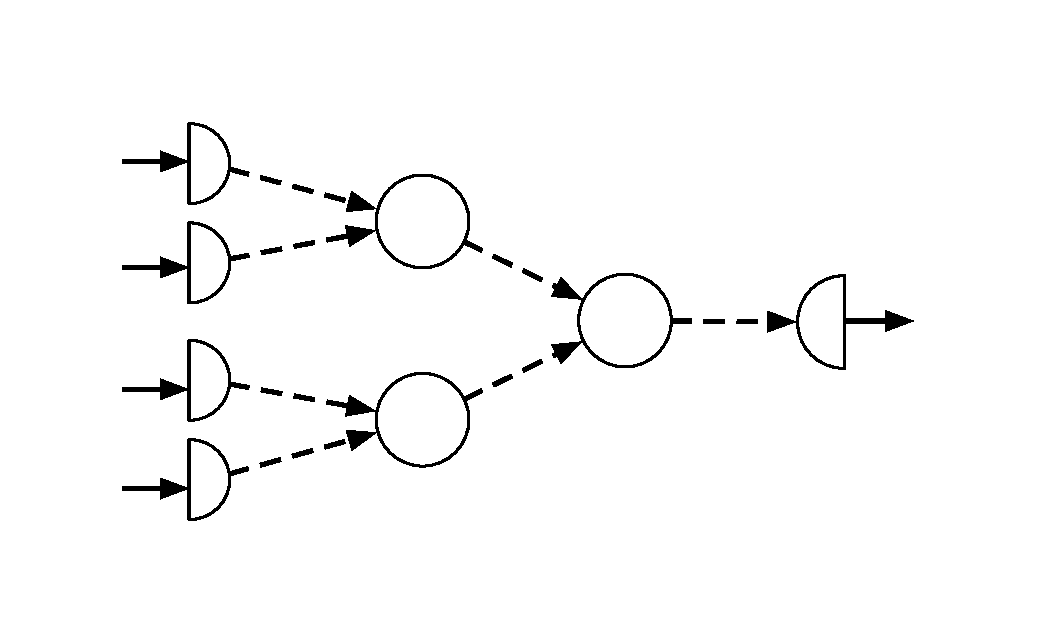
\includegraphics[width=3cm]{hadoop2}%
\end{center}
}

\usepackage{tikz}
\usetikzlibrary{shadows.blur}
\usetikzlibrary{shapes.symbols}
\usetikzlibrary{backgrounds}
\usetikzlibrary{arrows.meta}
\usetikzlibrary{shapes,snakes}
\usetikzlibrary{fit,calc,shadows}
\setbeamercolor{section in head/foot}{bg=white, fg=black}
%\beamertemplateshadingbackground{black!10}{blue!15}
\makeatletter
\setbeamertemplate{footline}
{
  \leavevmode%
  \hbox{%
  \begin{beamercolorbox}[wd=.333333\paperwidth,ht=2.25ex,dp=1ex,center]{section in head/foot}%
    \usebeamerfont{author in head/foot}\insertshortauthor~~\beamer@ifempty{\insertshortinstitute}{}{Richard G. Clegg}
  \end{beamercolorbox}%
  \begin{beamercolorbox}[wd=.333333\paperwidth,ht=2.25ex,dp=1ex,center]{section in head/foot}%
    \usebeamerfont{title in head/foot}{Creating synthetic networks}
  \end{beamercolorbox}%
  \begin{beamercolorbox}[wd=.333333\paperwidth,ht=2.25ex,dp=1ex,right]{section in head/foot}%
    \usebeamerfont{date in head/foot}\insertshortdate{}\hspace*{2em}
    \insertframenumber{} / \inserttotalframenumber\hspace*{2ex} 
  \end{beamercolorbox}}%
  \vskip0pt%
}


\tikzstyle{cloudconn} = [draw=black, inner sep=0pt,
       line width=0.25mm,{Latex[length=2.5mm, width=1.5mm]}-{Latex[length=2.5mm, width=1.5mm]}]

\tikzstyle{arrowconn} = [draw=black, inner sep=0pt,
       line width=0.25mm,-{Latex[length=2.5mm, width=1.5mm]}]
\makeatother

\date[Covid 2021 workshop]{Presentation Covid 2021 workshop}

\begin{document}


\frame{

\title[Synthetic networks]{Freeing vital research with synthetic network data}

\setcounter{framenumber}{0}

\begin{center}
\Huge{Creating‌ ‌synthetic‌ ‌models‌ ‌from‌ ‌sensitive‌ ‌data‌: \\ ‌ ‌preparing‌ ‌for‌ ‌future‌‌ epidemics}


\vspace{0.2cm}

\inserttitlegraphic

\vspace{0.2cm}

\scriptsize{\raggedright
{\color{blue} Presenter: }Richard G. Clegg  \\
    {\color{blue} FETA written by Naomi A. Arnold and Richard G. Clegg}
}

\tiny{(Prepared using \LaTeX \;and beamer.)}
\end{center}
}

\tikzset{onslide/.code args={<#1>#2}{%
  \only<#1>{\pgfkeysalso{#2}} % \pgfkeysalso doesn't change the path
}}
\tikzset{temporal/.code args={<#1>#2#3#4}{%
  \temporal<#1>{\pgfkeysalso{#2}}{\pgfkeysalso{#3}}{\pgfkeysalso{#4}} % \pgfkeysalso doesn't change the path
}}

\tikzstyle{platform} = [draw=black,shade, 
      anchor=south west,
      align= center,
      top color=blue!40,
      bottom color=blue!5,
      rounded corners=6pt,
      blur shadow={shadow blur steps=5},
      font = \footnotesize]

\section{Introduction}


\tikzstyle{box} = [draw=black,shade, 
      font = \footnotesize,
      align= center,
      top color=blue!40,
      bottom color=blue!5,
      rounded corners=3pt,
      blur shadow={shadow blur steps=5}]

\tikzstyle{box2} = [draw=black,shade, 
      font = \footnotesize,
      align= center,
      top color=red!40,
      bottom color=red!5,
      rounded corners=3pt,
      blur shadow={shadow blur steps=5}]

\tikzstyle{net con} = [draw=black,ultra thick,->]


\frame{
    
    \frametitle{Synthetic network data: The problem}
\begin{block}{Isle of Wight Covid App data}
May 2020: trial UK Covid tracking app released on the Isle of Wight.  \\
Data collected: when users encountered each other (network of encounters), when people tested positive for Covid (spread of disease over network). 
\end{block}
\pause
\begin{block}{Invaluable network data that can never be used}
Uses: Understanding disease spread, understanding transmission network, tuning covid app, testing vaccine strategies. \\ 
If researchers had access could revolutionise understanding.
\end{block}
\pause
\begin{itemize}
\item Imagine a world where everyone who built a centralised Covid tracing app could also release a `best possible' privacy preserving version of the contact network with no privacy concerns.  
\end{itemize}

}



\definecolor{lavander}{cmyk}{0,0.48,0,0}
\definecolor{violet}{cmyk}{0.79,0.88,0,0}
\definecolor{burntorange}{cmyk}{0,0.52,1,0}

\def\lav{lavander!90}
\def\oran{orange!30}

\tikzstyle{peers}=[draw,circle,violet,bottom color=\lav,
                  top color= white, text=violet,minimum width=10pt]
\tikzstyle{superpeers}=[draw,circle,burntorange, left color=\oran,
                       text=violet,minimum width=10pt]
\tikzstyle{legendsp}=[rectangle, draw, burntorange, rounded corners,
                     thin,bottom color=\oran, top color=white,
                     text=burntorange, minimum width=1.5cm]
\tikzstyle{legendp}=[rectangle, draw, violet, rounded corners, thin,
                     bottom color=\lav, top color= white,
                     text= violet, minimum width= 1.5cm]
\tikzstyle{legend_general}=[rectangle, rounded corners, thin,
                           burntorange, fill= white, draw, text=violet,
                           minimum width=1.5cm, minimum height=0.4cm]

\tikzfading[name=arrowfading, top color=transparent!0, bottom color=transparent!95]
\tikzset{arrowfill/.style={#1,general shadow={fill=black, shadow yshift=-0.8ex, path fading=arrowfading}}}
\tikzset{arrowstyle/.style n args={3}{draw=#2,arrowfill={#3}, single arrow,minimum height=#1, single arrow,
single arrow head extend=.3cm,}}

\NewDocumentCommand{\tikzfancyarrow}{O{2cm} O{FireBrick} O{top color=OrangeRed!20, bottom color=Red} m}{
\tikz[baseline=-0.5ex]\node [arrowstyle={#1}{#2}{#3}] {#4};
}


\frame{
\frametitle{Synthetic network data: high level description}


\begin{block}{Synthetic network data}
\begin{itemize}
\item Take an original \alert{target} network.
\item Find algorithmic construction rules that match this network.
\item Grow network (or networks) from these rules.
\end{itemize}
\end{block}

\begin{tikzpicture}
\draw[white] (-2,-3) rectangle (10,2);
\node <2-> at (-0.2,0) {
\begin{minipage}{0.8\textwidth}
\begin{tikzpicture}[auto, thick]
 
  % Place super peers and connect them
  \foreach \place/\name in {{(0,-0.5)/a}, {(1,0)/b}, {(1,1)/c}, {(0,1)/d},
           {(-1,0)/e}}
    \node[superpeers] (\name) at \place {};
  \foreach \source/\dest in {a/b, a/c, a/d, b/c, c/d,a/e,d/e}
    \path (\source) edge (\dest);
   %
   % Place normal peers
  \foreach \pos/\i in {above left of/1, left of/2, below left of/3}
    \node[peers, \pos = e] (e\i) {};
   \foreach \speer/\peer in {e/e1,e/e2,e/e3}
    \path (\speer) edge (\peer);
   %
   %
   \foreach \pos/\i in {above right of/1, right of/2, below right of/3}
    \node[peers, \pos =b ] (b\i) {};
   \foreach \speer/\peer in {b/b1,b/b2,b/b3}
   \path (\speer) edge (\peer);
   %
   \node[peers, above of=d] (d1){};
   \path (d) edge (d1);
   %
   \foreach \pos/\i in {below left of/1, below of/2}
   \node[peers, \pos =a ] (a\i) {};
   \foreach \speer/\peer in {a/a1,a/a2}
   \path (\speer) edge (\peer);
\end{tikzpicture}
\end{minipage}
};

\node<3-> at (1,0) {
\tikzfancyarrow[3cm]{$p_i = k d_i^{\alpha}$}

};

\node <4-> at (7.5,0) {
\begin{minipage}{0.8\textwidth}
\begin{tikzpicture}[auto, thick]
  % Place super peers and connect them
  \foreach \place/\name in {{(0,-0.4)/a}, {(0.9,0.2)/b}, {(0.7,1.3)/c}, {(0.3,1.2)/d},
           {(-1.2,0.3)/e}}
    \node[superpeers] (\name) at \place {};
  \foreach \source/\dest in {a/b, a/c, a/d, b/c, c/d,a/e,d/e}
    \path (\source) edge (\dest);
   %
   % Place normal peers
  \foreach \pos/\i in {above left of/1, left of/2}
    \node[peers, \pos = e] (e\i) {};
   \foreach \speer/\peer in {e/e1,e/e2}
    \path (\speer) edge (\peer);
   %
   %
   \foreach \pos/\i in {above right of/1, right of/2}
    \node[peers, \pos =b ] (b\i) {};
   \foreach \speer/\peer in {b/b1,b/b2}
   \path (\speer) edge (\peer);
   %
   \node[peers, above of=d] (d1){};
   \path (d) edge (d1);
   %
   \foreach \pos/\i in {below left of/1, below right of/2}
   \node[peers, \pos =a ] (a\i) {};
   \foreach \speer/\peer in {a/a1,a/a2}
   \path (\speer) edge (\peer);
\end{tikzpicture}
\end{minipage}
};

\end{tikzpicture}

}


\frame{
    \frametitle{Alternatives to synthetic network data?}
\centering{
\begin{tikzpicture}%[show background grid]
\draw[white] (-5.5,-3.5) rectangle (5.5,3.5);
\node <1-> at (0,0) {
\begin{minipage}{0.8\textwidth}
\begin{block}{Anonymise}
Release the data anonymised so there are no privacy concerns. \\
Allows data to be open and available for research.
\end{block}

    
\begin{block}{Guarantee to keep data secure}
Release data to individual researchers under an NDA (non disclosure agreement). 
\end{block}
\pause
These routes to sharing data present clear danger with the most private (most valuable) data.
Network data is incredibly hard to anonymise well. 
\end{minipage}
};

\node <3-> at (-2,0) {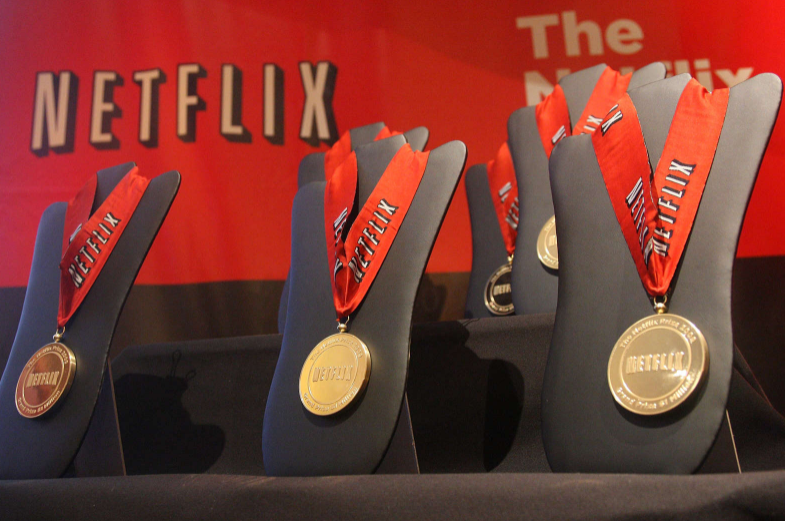
\includegraphics[width=7cm,angle=20]{netflix_prize}};
\node <4-> at (2,2) {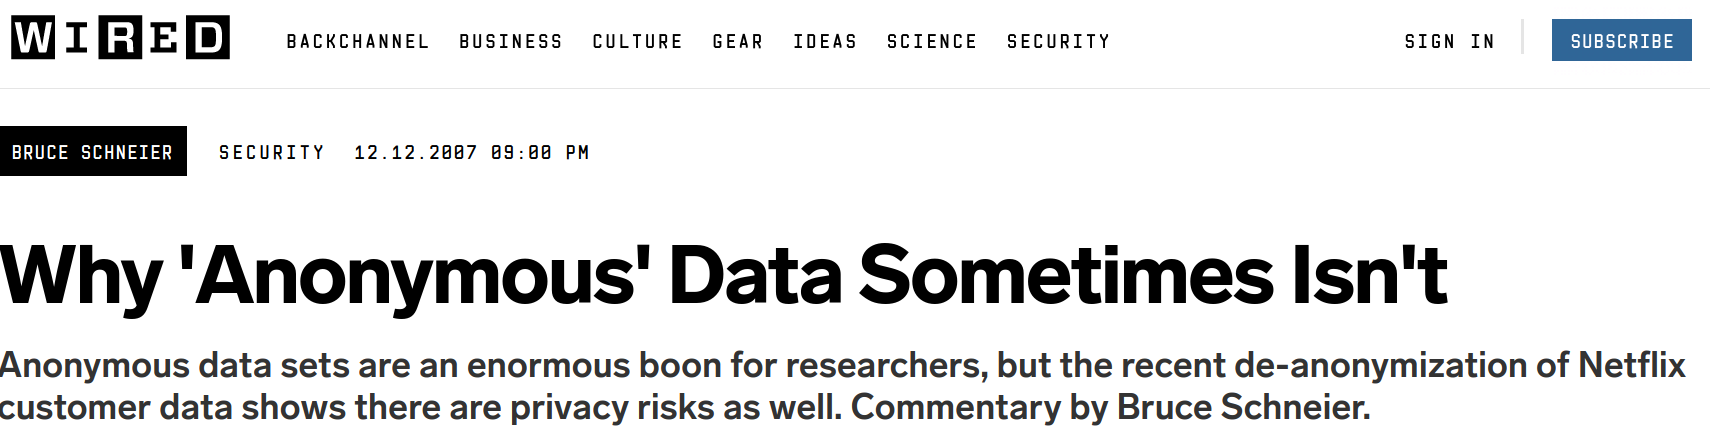
\includegraphics[width=8cm,angle=-10]{wired_netflix}};
\node <5-> at (-1,0) {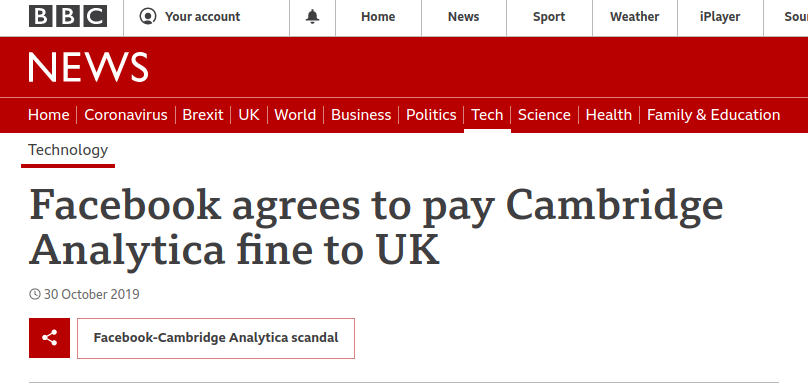
\includegraphics[width=8cm,angle=-30]{camb_priv}};
\node <6-> at (0,0) {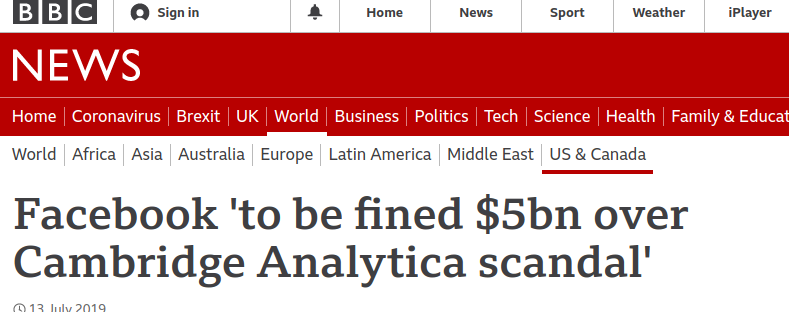
\includegraphics[width=6cm,angle=40]{camb_priv2}};
\end{tikzpicture}

}

}


\frame{
\frametitle{Synthetic temporal networks to share private network data}

\begin{block}{Replicating target temporal network}
Want to create a probabilistic model giving rules to construct a network that has ``the same properties" but is ``low parameter" (cannot leak much information). 
\end{block}

\begin{block}{Why temporal networks?}
Timestamps and arrival order gives more information to work with. Existing body of work on growing network models. 
\end{block}

\begin{block}{Static networks}
A few possible approaches exist, for example Exponential Random Graph models. 
\end{block}
}

\frame{
\frametitle{Synthetic temporal networks -- the ideal solution}
\centering{
\begin{tikzpicture}%[show background grid]
\draw[white] (-1,-1) rectangle (10,7);
\node<1->[box] at (0.5,6.5) (targ){Target Network \\ for synthesis};
\node<1->[box] at (4.5,6.5) (soft){Analysis software};
\draw<1-> [net con] (targ) -- (soft);
\node<2->[box] at (4.5,3.5) (opt){Optimal\\ temporal model};
\draw<2-> [net con] (soft) -- (opt);
\node<3->[box] at (8.5,3.5) (net){Generated \\ synthetic network};
\draw<3-> [net con] (opt) -- (net);
\draw<4-> [black, fill=green,opacity=0.2] (-1,7.0) rectangle (6.5,5.5);
\node<4-> at (1,5.7) {Stays private};
\draw<4-> [black, fill=blue,opacity=0.2] (3,5) rectangle (10,2);
\node<4->  at (7,2.8) {Released to world};
\node<4->  at (6.8,2.4) {(10s/100s bits of info)};
\node<5-> [box] at (8.5,1.0) (res) {Research algorithms \\tested};
\draw<5-> [net con] (net) -- (res);
\node<6-> [box] at (0.5,1.0) (sol) {Optimal solutions \\ fed back};
\draw<6-> [net con] (res) -- (sol);
\draw<6-> [net con] (sol) -- (targ);
\end{tikzpicture}
}
}

\frame{
\frametitle{Structure of temporal models}

\begin{block}{Probabilistic models}
Let $\bG= (G_i, G_{i+1}, \ldots, G_{i+n})$ be random variables
representing the evolution of a graph observed at discrete times with $g_i$ being an observation of $G_i$. Valid models specify $\Prob{G_{t+1} = g_{t+1} | 
G_t=g_t, G_{t-1} = g_{t-1},\ldots}$
\end{block}

\begin{itemize}
\item Rules in models with ordered node arrivals like: 
\begin{itemize}
\item Barab{\'a}si--Albert, Bianconi--Barab{\'a}si model, Temporal Preferential Attachment
\item Jackson--Rogers model (completing friendship triangles)
\end{itemize}
\item Rules out models without ordered node arrivals like:
\begin{itemize}
\item Randomised Reference models
\item Erd\H{o}s-R\'{e}nyi, Stochastic Block model
\item Exponential Random Graph models
\end{itemize}
\end{itemize}

}


\frame{
\frametitle{Sub-dividing the temporal network problem}
\begin{block}{Operation model}
\begin{itemize}
\item Process to select an operation on the network.
\item Could be: \alert{add node}, 
\alert{add edge}, 
\alert{remove node} and so on.
\end{itemize}
\end{block}

\begin{block}{Object model}
\begin{itemize}
\item Process selects which nodes/edges are involved in operation
selected by operation model.
\item Probabilities are assigned to nodes and potential
edges for random selection.
\item Edges selected by assigning probabilities to node pairs.
\end{itemize}
\end{block}
}

\frame{
\frametitle{Commentary on Operation and Object model}

\begin{itemize}
\item The object model is given a lot of attention in networks literature.
\item BA model synonymous with preferential attachment, forget $m=3$. 
\item Operation model is rarely studied yet governs vital network parameters e.g. $\langle k \rangle$.
\item Typical operation model in the literature will produce a fixed node-edge ratio.
\end{itemize}
\centering{
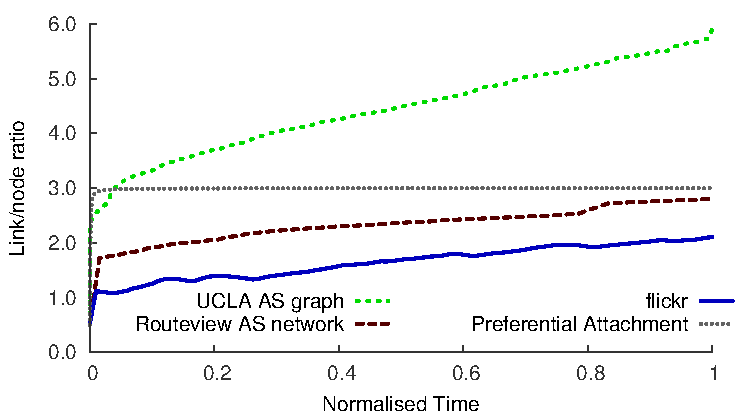
\includegraphics[width=10cm]{link_node_evolve} \\
}
}

%\frame{
%\frametitle{Synthetic network data -- some current approaches}

%\begin{block}{Link Data Benchmark Council}
%LDBC widely used industry standard for synthetic social networks. Software produces synthetic social network data with information about users/posts but with extremely simple graph structure aimed at benchmarking.
%\end{block}

%\begin{block}{Complex networks based models}
%Based on sound mathematical principles. Examples:
%\begin{itemize}
%\item Random (Erd\H{o}s--Renyi) -- connect new nodes at random.
%\item Barab\'{a}si--Albert -- connect new nodes with a probability proportional to node degree.
%\item Triangle closure (Jackson) -- connect new node to a random node and a ``friend" of that random node. 
%\end{itemize}
%Interesting, mathematically tractable, but do not capture the complexities of real world networks.
%\end{block}
%}



\frame{
\frametitle{FETA: Framework for Evolving Topology Analysis}
\centering{
\begin{tikzpicture}
\node at (0,0) {\begin{minipage}{\textwidth}
\begin{block}{Creates networks from mixtures of models}
Example: model is 50\% Barab\'{a}si--Albert and 50\% Random. These mixtures can vary in time.
\end{block}

\begin{block}{Assess mathematical likelihood against a target observed network}
Which mixture of models $X$, $Y$ and $Z$ is most likely as an explanation of observed network $N$?
Is the model improved if this mixture changes in time?
\end{block}

\begin{block}{Easily allow development of new network model components}
Quick to add in new models for testing. They can then be combined as with the other model components.
\end{block}
\end{minipage}
};
\node<2->[] at (-3.0,-1.2) {
\begin{minipage}{0.5\textwidth}
\pgfmathsetseed{23654}
\begin{tornpage}    
    Likelihood based assessment of Dynamic Networks\\
    \bf{J. Network Sci. 2016}
\end{tornpage}
\end{minipage}};
\node<3->[] at (3.0,-1.2) {
\begin{minipage}{0.5\textwidth}
\pgfmathsetseed{23654}
\begin{tornpage}    
    Likelihood based approach to discriminate mixtures
    of network models...\\
    \bf{Nature Sci. Rep 2021}
\end{tornpage}
\end{minipage}};
\node<4->[] at (0,2) {
\begin{minipage}{0.5\textwidth}
\pgfmathsetseed{23654}
\begin{tornpage}    
    Open source software\\
    \bf{github.com/narnolddd/FETA3}
\end{tornpage}
\end{minipage}};
\end{tikzpicture}
}
}

\frame{
\frametitle{Producing synthetic networks with FETA}
\centering{
\begin{tikzpicture}%[show background grid]
\draw[white] (-1,-1) rectangle (10,7);
\node<1->[box] at (0.5,6.5) (ba) {Barab{\'a}si--Albert \\ model};
\node<1->[box] at (4.5,6.5) (er) {Random model};
\node<1->[box] at (8.5,6.5) (tri) {Triangle model};
\node<1->[box] at (0.5,3.0) (targ){Target Network \\ for synthesis};
\node<2->[box] at (4.5,3.0) (feta){FETA analysis};
\draw<2-> [net con] (ba) -- (feta);
\draw<2-> [net con] (er) -- (feta);
\draw<2-> [net con] (tri) -- (feta);
\draw<2-> [net con] (targ) -- (feta);
\node<3->[box] at (4.5,0.5) (opt){Maximally likely\\ model combination};
\draw<3-> [net con] (feta) -- (opt);
\node<4->[box] at (8.5,0.5) (net){Synthetic network \\ generation};
\draw<4-> [net con] (opt) -- (net);
\draw<5-> [black, fill=green,opacity=0.2] (-1,4.5) rectangle (6,2.5);
\node<5-> at (1,4) {Stays private};
\draw<5-> [black, fill=blue,opacity=0.2] (3,2) rectangle (10,0);
\node<5-> at (7,1.7) {Released to world};
\node<5-> at (6.8,1.3) {(10s/100s bits of info)};
\end{tikzpicture}
}
}
\frame{
\frametitle{The likelihood of FETA model}
\begin{itemize}
\item Let $M(\btheta)$ be a parameterised FETA model with parameters $\btheta$.
\item Define $f_{i}(g_i)= \Prob{G_{i}=g_i| M(\btheta), G_{i-1}=g_{i-1}, 
G_{i-2}=g_{i-2}, \ldots}$.
\item Given the observations $\bg=(g_i, g_{i-1}, \ldots, g_1)$, the likelihood of the model $M(\btheta)$ is given by: \\
$L(M(\btheta) | \bg ) = \prod_{k=i+1}^{k=i+n} f_k(g_k)$.
\item This is the likelihood that the observations arose from the proposed model. 
\item This ability to assign true likelihood to the
graph evolution which is key to the FETA process.
\end{itemize}
}

\frame{
\frametitle{Object model components}
Throughout $k$ is a normalising constant such that $\sum_i p_i = 1$
for all nodes considered.  
$p_i$ is the probability of picking node
$i$ (at the stage being considered).

\begin{itemize}
\item Random model $M_0 \quad p_i = 1/k$.
\item Preferential attachment $M_d \quad p_i = d_i /k$.
\item PFP $M_p(\delta) \quad p_i = d_i^{1+\delta \log_{10} (d_i)}/k$  where $\delta$ is a parameter.
\item Degree power $M_d(\alpha) \quad p_i = d_i^{\alpha}/k$ where $\alpha$ is a parameter.
\item Triangle model $M_t(N) = 1/k$ if node in neighbourhood of $N$ most recently chosen.
\item Singleton model $M_1(N) = 1/k$ if node has degree 1 $0$ otherwise.
\item Doubleton model $M_2(N) = 1/k$ if node has degree 2 $0$ otherwise.
\end{itemize}
}


\section {Testing FETA}

\subsection{Artificial tests}

\frame{
\frametitle{Artificial tests}
\begin{itemize}
\item Perhaps the most convincing test of such a model is its ability to
recover parameters from a known model.
\item Create a realisation of a graph with known $M(\btheta)$.  
\item From this graph try to recover $\btheta$ with maximum likelihood.
\item Linear parameters of model can be assessed ``in parallel" (model tracks likelihood for a range of answers simultaneously).
\item Other (non-linear) parameters can be found from ``parameter sweeps" 
(assessing the likelihood for many values of that parameter).
\item Look at a measure $c_0$ which gives a ``human readable" likelihood relative to a null model of ``random" connections.
\end{itemize}
}

\frame{
\frametitle{Sweep one parameter (10,000 link network)}
\centering{
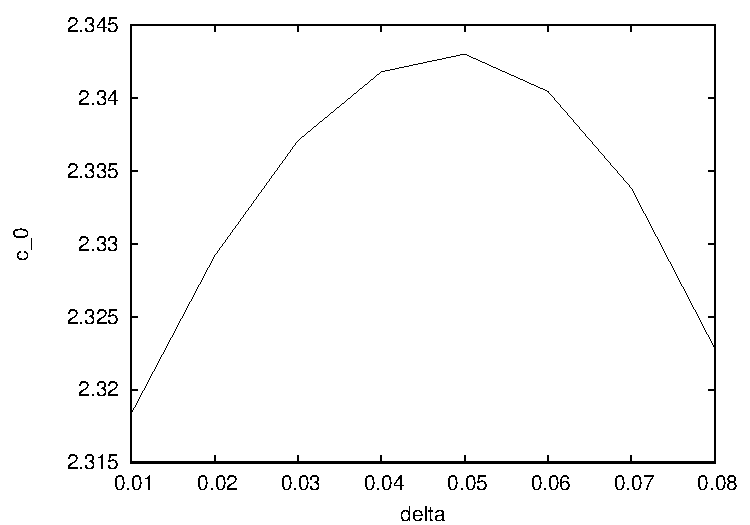
\includegraphics[width=10cm]{deltasweep} \\
}
PFP model $M= M_p(0.05)$.  Correct answer is $\delta = 0.05$.
}

\frame{
\frametitle{Sweep two parameters (10,000 link network)}
\centering{
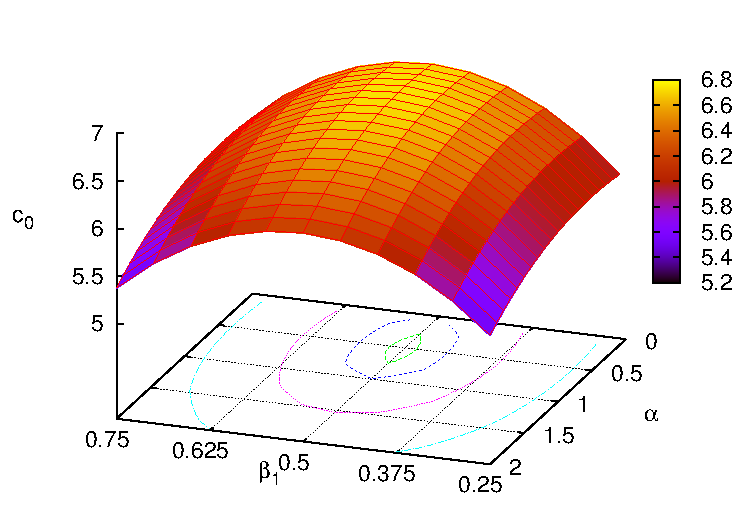
\includegraphics[width=8cm]{art1_data} \\
}
Correct model $M = 0.5 M_2 + 0.5 M_d(0.5)$
fitted $M= \beta_1 M_2 + (1-\beta_1) M_d(\alpha)$.
}


\frame{
\frametitle{Models which change in time -- artificial data}
\begin{itemize}
\item Model changes once at time $T$.  Use the ``degree power" model and change the power.
\item Let $p_i(t)$ be the probability of choosing $i$ at time $t$.
\item Let $d_i(t)$ be the degree of $i$ at time $t$.
$$p_i(t) =
\begin{cases} d_i(t)^\alpha/k & t < T \\
d_i(t)^\beta/k & t \geq T.
\end{cases} 
$$
\item Now we can grow a graph using this model for different $\alpha$ and $\beta$.
\item Already shown for a long section of data we can recover the parameter.
\item Can we locate the point at which the change occurs?
\end{itemize}
}

\subsection{Finding the change point}


\frame{
\frametitle{Finding the change point -- 10000 node experiment}
\begin{center}
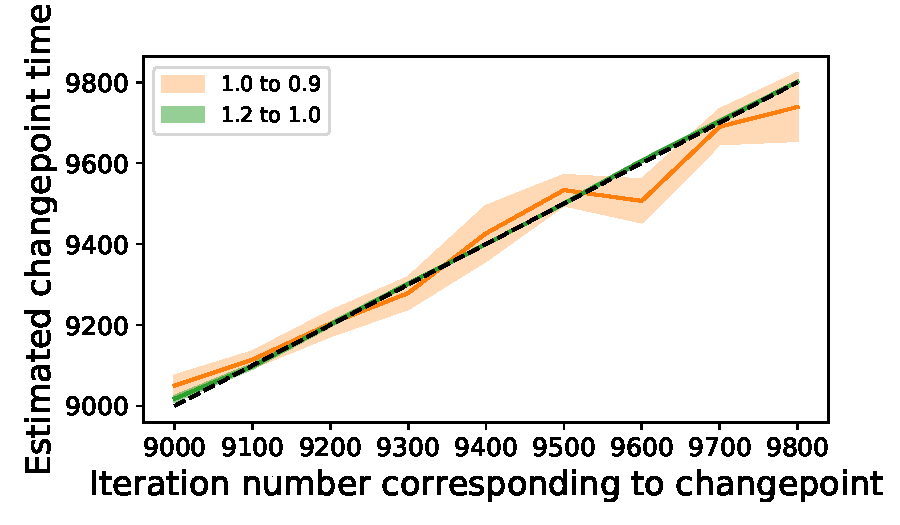
\includegraphics[height=0.8\textheight]{DP10000_diff_markers}
\end{center}
}

\frame{
\frametitle{Critical assessment of FETA to generate synthetic network}

\begin{block}{Solves half the problem fairly well}
\begin{itemize}
\item Tell which of a set of models (and linear combination of models) has highest likelihood.
\item Correctly recovers parameters for artificial models (even close models that produce the same degree distribution). 
\item Finds the most likely set of change points for models that change in time.
\end{itemize}
\end{block}

\begin{block}{Fails to solve other important problems}
\begin{itemize}
\item Fails to capture clustering and assortativity on most data sets.
\item Requires considerable user intervention.
\item Tells you nothing about the operation model (we \alert{cheat} and clone it). 
\end{itemize}
\end{block}
}

\frame{
\frametitle{Conclusion: path to producing synthetic network models}

\begin{itemize}
\item Alternative approaches for the ``object" model exist.
\begin{itemize}
\item ``Choosing to grow a graph", Overgoor, Benson, Ugander 2020 is somewhat similar but uses a logit framework for links as choices.
\item ``Clustering and preferential attachment in growing networks" Newman, 2001 works for a restricted set of models.
\end{itemize}
\item None of these including FETA yet work as software that a user can easily work with to get the ``best possible" synthetic network.
\item The ``operation model" part of this does not seem to have attracted much attention.
\begin{itemize}
\item These models quickly become analytically intractable but the detail given is vital for an accurate network model. 
\item In modelling pandemics, the number of contacts added and the time order are extremely critical. 
\end{itemize}
\item For the next pandemic we want to be able to say to a person with confidential infection network data: \alert{``This software will produce the best possible synthetic version that preserves privacy."} We cannot do that today.
\end{itemize}

}



\appendix
\backupbegin

\frame{
\frametitle{FETA analysis of Enron email network}
\centering{
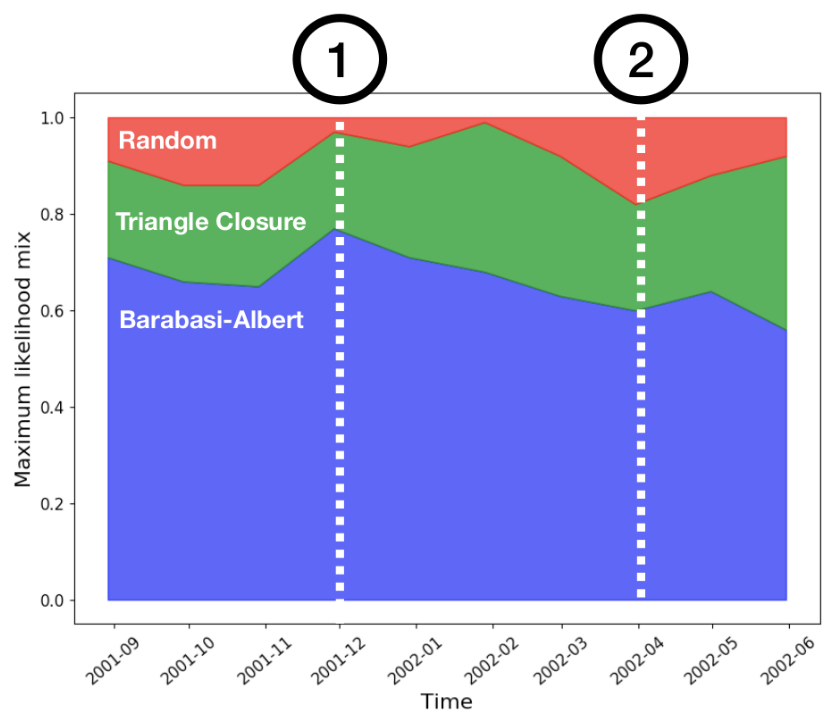
\includegraphics[height=0.7\textheight]{enron}
\begin{enumerate}
\item Enron files for bankruptcy.
\item Auditor pleads guilty of obstruction.
\end{enumerate}
}
}
\backupend

\end{document}
